\documentclass{article}
\usepackage{tikz}
\usepackage{tkz-euclide}
\definecolor{darkgreen}{RGB}{0,192,0}
\title{Cartesian closed categories and the price of eggs}
\author{Jane Doe}
\date{September 1994}
\begin{document}

	\begin{figure}
		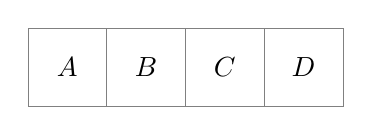
\begin{tikzpicture}
			\draw[step=1cm,gray,very thin] (0,0) grid (4,1);
			\draw (0.5,0.5) node {$A$};
			\draw (1.5,0.5) node {$B$};
			\draw (2.5,0.5) node {$C$};
			\draw (3.5,0.5) node {$D$};
		\end{tikzpicture}

		\vspace{5mm}

		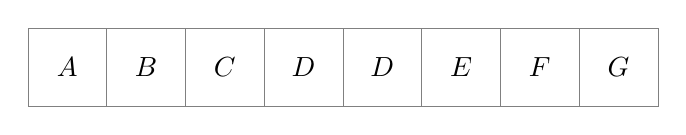
\begin{tikzpicture}
			\draw[step=1cm,gray,very thin] (0,0) grid (8,1);
			\draw (0.5,0.5) node {$A$};
			\draw (1.5,0.5) node {$B$};
			\draw (2.5,0.5) node {$C$};
			\draw (3.5,0.5) node {$D$};
			\draw (4.5,0.5) node {$D$};
			\draw (5.5,0.5) node {$E$};
			\draw (6.5,0.5) node {$F$};
			\draw (7.5,0.5) node {$G$};			
		\end{tikzpicture}		
		\caption{\textit{Top:} A cubic curve with control points $A,B,C,D$ encoded in a 1d texture.  \textit{Bottom:} Two piecewise curves encoded in a 1d texture.  The control points for the first curve are $A,B,C,D$ and the control points for the second curve are $D,E,F,G$.  If C0 continuitiy is always desired between the curves, a redundant $D$ could be removed to store these curves in 7 pixels instead of 8.}		
		\label{fig:texlayeout1d}
	\end{figure}	

\end{document}